\Class{Fighter}
{Any wastelander can pick up a bone and call it a club, but try pitting fifty of those against one dozen trained soldiers, and maybe you'll have an even match.}{Nikolos, human fighter}

From the small forts in sandy wastes of Athas to the guards of the merchant houses in the city-states, fighters are Athas' most common sight. Whether it is as mercenaries for the sorcerer-kings or as hired guards protecting the wealth of the nobility, fighters can be found everywhere in the Tablelands. Athas' fighters are trained to fight in small groups or huge units. Those that have proven themselves become the commanders in the city-states' armies, commanding hundreds or even thousands of men into war.

\begin{figure}[b!]
\centering
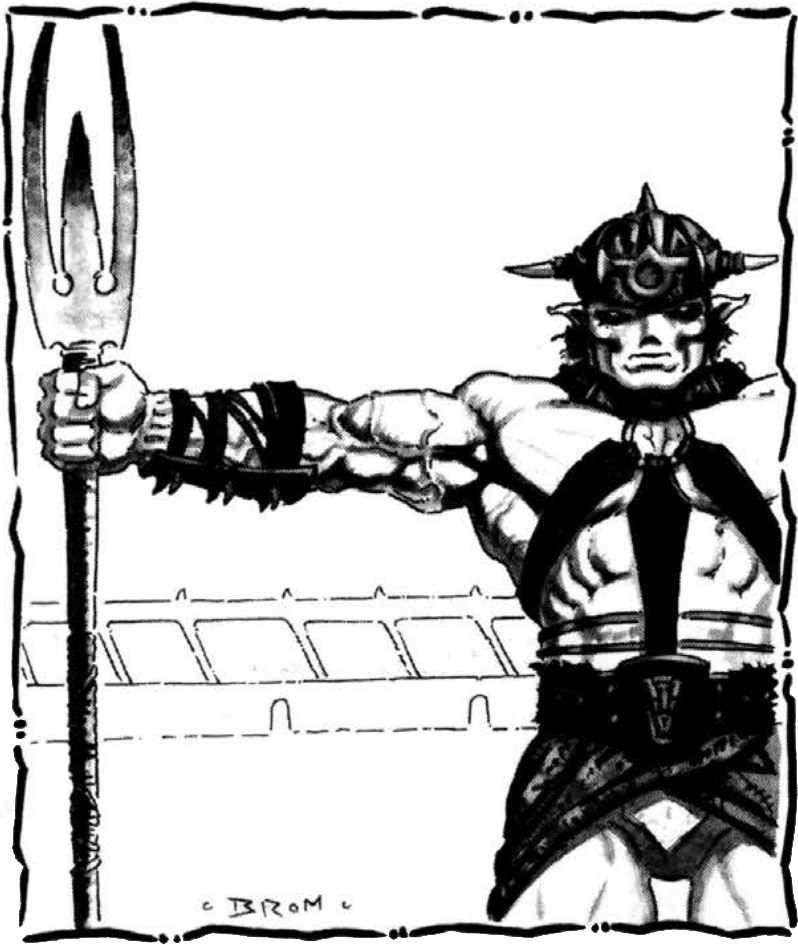
\includegraphics[width=\columnwidth]{images/gladiator-1.png}
\end{figure}

\subsection{Making a Fighter}

Fighters receive the best allotment of fighting skills and abilities. They learn the use of most weapons, the best armors and shields, as well as gaining special abilities to use with these weapons and armor.

Some fighters specialize in using a single weapon, and become masters at its use and deadliness. Other fighters will prefer more rounded skills, learning to shoot from far with bows and arrows, or nets or spears. Regardless, the fighter is to be feared.

\textbf{Races:} All of Athas' races can become fighters. Humans are usually the most numerous, though, since they are the most numerous of the races of the Tablelands. Dwarves make good fighters, even though they are smaller than most races; their inborn toughness and great strength more than makes up for their smaller stature. The half-giants are also seen very often as fighters, since their great strength and size are perfect for the job. Muls, with the inherited traits of both humans and dwarves, are also great fighters. Elves, with their long legs and frail constitution, are not often seen as fighters. Athas' intelligent insects, the Thri-kreen, make excellent warriors, with their four arms and the fact they do not need to sleep. Many of the savage races of the Tablelands are fighters, although most become rangers in order to survive.

\textbf{Alignment:} Fighters come from all walks of life, and can be of any alignment. Good fighters are usually seen as the protectors of small villagers or are part of renegade slave tribes, helping their tribe to survive in the harsh desert. Or they can be found as a dwarf perhaps, whose focus it is to guard his fellows. Evil fighters are often part of mercenary bands or under the control of a sorcerer-king; these beings often fight for power and money. Evil fighters can also be found as the rulers of small forts, guarding their oasis and exacting a hefty toll for its use.

\MiniWarriorTable{The Fighter}{
1 & +1 & +2 & +0 & +0 & Bonus feat \\
2 & +2 & +3 & +0 & +0 & Bonus feat \\
3 & +3 & +3 & +1 & +1 &  \\
4 & +4 & +4 & +1 & +1 & Bonus feat \\
5 & +5 & +4 & +1 & +1 &  \\
6 & +6/+1 & +5 & +2 & +2 & Bonus feat \\
7 & +7/+2 & +5 & +2 & +2 &  \\
8 & +8/+3 & +6 & +2 & +2 & Bonus feat \\
9 & +9/+4 & +6 & +3 & +3 &  \\
10 & +10/+5 & +7 & +3 & +3 & Bonus feat \\
11 & +11/+6/+1 & +7 & +3 & +3 &  \\
12 & +12/+7/+2 & +8 & +4 & +4 & Bonus feat \\
13 & +13/+8/+3 & +8 & +4 & +4 &  \\
14 & +14/+9/+4 & +9 & +4 & +4 & Bonus feat \\
15 & +15/+10/+5 & +9 & +5 & +5 &  \\
16 & +16/+11/+6/+1 & +10 & +5 & +5 & Bonus feat \\
17 & +17/+12/+7/+2 & +10 & +5 & +5 &  \\
18 & +18/+13/+8/+3 & +11 & +6 & +6 & Bonus feat \\
19 & +19/+14/+9/+4 & +11 & +6 & +6 &  \\
20 & +20/+15/+10/+5 & +12 & +6 & +6 & Bonus feat}

\subsection{Game Rule Information}
\textbf{Hit Die:} d10.

\subsubsection{Class Skills}
\skill{Climb} (Str), \skill{Craft} (Int), \skill{Handle Animal} (Cha), \skill{Intimidate} (Cha), \skill{Jump} (Str), \skill{Knowledge} (warcraft) (Int), and \skill{Ride} (Dex).

\textbf{Skill Points per Level:} 2 + Int modifier ($\times4$ at 1st level).

\subsubsection{Class Features}

\textbf{Weapon and Armor Proficiency:} A fighter is proficient with all simple and martial weapons and with all armor (heavy, medium, and light) and shields (including tower shields).

\textbf{Bonus Feats:} At 1st level, a fighter gets a bonus combat-oriented feat in addition to the feat that any 1st-level character gets and the bonus feat granted to a human character. The fighter gains an additional bonus feat at 2nd level and every two fighter levels thereafter (4th, 6th, 8th, 10th, 12th, 14th, 16th, 18th, and 20th). These bonus feats must be drawn from the feats noted as fighter bonus feats. A fighter must still meet all prerequisites for a bonus feat, including ability score and base attack bonus minimums.

These bonus feats are in addition to the feat that a character of any class gets from advancing levels. A fighter is not limited to the list of fighter bonus feats when choosing these feats.

\subsection{Playing a Fighter}

Playing an Athasian fighter is not much different than playing one in other settings, the only difference is that the extreme heat makes most armor less than desirable on Athas.

As a fighter, you undertake adventures according to the dictates of your cause, your faith, or your own selfish needs. You might find yourself on the hot, sandy field of battle, charging shoulder to shoulder with peasants and soldiers, raising pitchforks and shields against the defilers of the enemy army.

\subsubsection{Religion}

There are no gods on Athas, but many fighters worship the sorcerer-king of their respective cities as gods. Some fighters pay homage to the elemental forces of the Tablelands, asking their favored element for luck before entering the battlefield.

\subsubsection{Other Classes}

Fighters get along with most other classes. The rangers of the Tablelands often receive the highest of the respect for their ability to survive the wastes. Gladiators and fighters are often at each other's throats, since both share great combat abilities but differ in their methodology; they often try to show how each is better than the other is. Elemental clerics are welcome for their healing abilities as well as the help they can provide in battle.

Fighters are uneasy around wizards; like the rest of the population they distrust magic. Templars are also distrusted, for the same reasons everyone else distrusts templars. Rogues are usually scorned by fighters; they prefer open battle to the rogue's sneaky ways.

\subsubsection{Combat}

Your specific tactics in battle depend on your role in the party and your weapon of choice. However, certain tactics are common to all fighters.

You are generally at the forefront of any battle. Fighting on the front line allows you maximize your combat feats. Furthermore, if opponents focus on you, they cannot injure your allies. As a fighter, you're at your best when you can take on the monster or opponent that deals the most damage.

\subsubsection{Advancement}

When looking at feats to select as you gain levels, you have two basic paths. You can focus on your fighting skills, or you can attempt to expand your capabilities to serve as the party's leader. The former option is best when you are the group's primary combat specialist. If the party includes another fighter or suitable melee character, you can afford to dabble in Charisma-based skills. Although Diplomacy is not a class skill for you, the Field Office feat combined with a few cross-class ranks makes you a serviceable emissary.

When it comes to combat feats, look to ones that improve your ability to deal damage. Feats such as Power Attack, Weapon Focus, and so forth are excellent options to boost your offense. Concentrated Fire, Rotate Lines, Shield Wall, and Spear Wall are excellent feats for army fighters.

Improved Initiative is a critically important feat, since it allows you to act first, move forward and defend or guide your allies. The sooner you find a place in the front line, the longer you can hold back the enemy.

\subsection{Starting Packages}

\subsubsection{The Archer}

Elf Fighter

\textbf{Ability Scores:} Str 15, Dex 16, Con 11, Int 10, Wis 12, Cha 8.

\textbf{Skills:} \skill{Jump}, \skill{Spot} (cc).

\textbf{Languages:} Common, Elven.

\textbf{Feat:} \feat{Point Blank Shot}, \feat{Precise Shot}.

\textbf{Weapons:} Macahuitl (1d8/19-20)

Dagger (1d4/19-20, 3 m)

Longbow with 40 arrows (1d8/$\times$3, 30 m).

\textbf{Armor:} Chitin armor (+4 AC).

\textbf{Gear:} Standard adventurer's kit, 11 cp.

\subsubsection{The Defender}

Dwarf Fighter

\textbf{Ability Scores:} Str 15, Dex 13, Con 16, Int 10, Wis 12, Cha 8.

\textbf{Skills:} \skill{Craft} (weaponsmithing), \skill{Knowledge} (warcraft), \skill{Intimidate}.

\textbf{Languages:} Common, Dwarven.

\textbf{Feat:} \feat{Disciplined}, \feat{Weapon Focus} (dwarven waraxe).

\textbf{Weapons:} Dwarven waraxe (1d10/$\times$3)

Shortbow with 20 arrows (1d6/$\times$3, 18 m).

\textbf{Armor:} Scale mail (+4 AC), heavy wooden shield (+2 AC).

\textbf{Gear:} Standard adventurer's kit, 42 cp.

\subsubsection{The Leader}

Human Fighter

\textbf{Ability Scores:} Str 15, Dex 8, Con 13, Int 10, Wis 12, Cha 14.

\textbf{Skills:} \skill{Diplomacy} (cc), \skill{Knowledge} (warcraft), \skill{Intimidate}.

\textbf{Languages:} Common.

\textbf{Feat:} \feat{Field Officer}, \feat{Inspiring Presence}, \feat{Weapon Focus} (great macahuitl).

\textbf{Weapons:} Great macahuitl (2d6, 19-20)

Shortbow with 20 arrows (1d6/$\times$3, 18).

\textbf{Armor:} Scale mail (+4 AC).

\textbf{Gear:} Standard adventurer's kit, 19 cp.

\subsection{Fighters on Athas}
\Quote[-.em]{Yeah, he was alright with a sword, but he would wet himself every time we walked out onto the sand of the arena. I think it was the crowd... or the goat-headed giant they paired us against. Poor little weed, he never saw that club coming.}{Grek the Grand, talking about his onetime matched pair contest with Slavek Thydor}

Fighters bring clashing weapons, stirring speeches, and mass combat to the campaign. On Athas, the fighter is a trained warrior, a soldier skilled in mass warfare. Every society on Athas maintains an army of fighters to protect itself from attack or to wage wars of plunder and annihilation against its neighbors. Fighters are both the commanders and soldiers in these armies, and at higher levels are experts in both individual and formation combat, leadership, and morale.

\subsubsection{Daily Life}

A fighter adventures to prove his superior skill at arms, to advance the cause of whatever master he might serve, and to further his own aims.

Once he has reached a respectable level of accomplishment, a fighter might take the Leadership feat and start building his own army. As word spreads, less experienced warriors who are eager to fight for the same causes seek him out as the desperate peoples of Athas constantly look for great commanders, warriors who will lead them.

\subsubsection{Notables}

Fighters can notoriety for their deeds, whether triumphs in combat, selfless acts of great honor, or great tyranny. Many an adventurer grew up on stories such as that of the Crimson Legion, and how it managed to defeat Urik's previously undefeated army.

Another legend tells of about the rise and fall of General Zanthiros, the leader of the Balican army who managed to save the city from an onslaught of beast-headed giants more than once, and after losing the elections, left the city with hundreds of soldiers loyal to him and formed a raiding tribe.

\subsubsection{Organizations}

Fighters often band together into small armies or as mercenary groups working for trade houses. These organizations typically have different credos and values, but they allow their members to focus their time on their individual quests.

\subsubsection{NPC Reactions}

Individuals react to fighters based on their previous interactions with other members of the class. A brave fighter meets cold silence and contempt around the Barrier Wastes where evil fighters oppress the populace.

Gladiators usually talk down on fighters, saying that gladiators are the true masters of combat. Fighters usually reply that gladiators are nothing without a crowd looking. Because of that, their initial reaction is one step towards unfriendly than normal.

A fighter who has lived long enough to retire from adventuring typically acquires some position of authority, with commensurate political power, whether as a caravan leader, army general, or ruler of a raiding or slave tribe.

\subsubsection{Fighter Lore}

Characters with ranks in \skill{Knowledge} (warcraft) can research fighters to learn more about them. When a character makes a skill check, read or paraphrase the following, including the information from lower DCs.

\textbf{DC 10:} Fighters may not be as flashy as gladiators in combat, but they surely are more effective in mass combat.

\textbf{DC 15:} Fighters are combat-oriented characters adept at hand-on-hand combat just as well as commanding entire armies.

\textbf{DC 20:} A fighter's mere presence in the battlefield can be enough to inspire his soldiers and weaken the resolve of his enemies.
